\documentclass[a4paper]{article}

\usepackage[margin=1in]{geometry} 
\usepackage[utf8]{inputenc}
\usepackage{hyperref}
\usepackage{graphicx, color}
\usepackage{lipsum}
\usepackage{natbib}
\usepackage[justification=centering]{caption}


% Research grant recipients must provide a summary report that is approximately two pages long, presenting the results of their funded research.  
% The report should include the status of the proposed work and note any significant changes from the initial proposal.
% The PI is expected to submit a summary report to the unit lead, Department Chair, Dean, Vice Provost for Research, and Provost.  

\title{Developing Data Pipelines for Research and Analysis}

\author{Seth Goodman$^1$\thanks{smgoodman@wm.edu} \and Jacob Hall$^1$ \and Cheyenne Hwang$^{1,2}$}

\date{
    $^1$AidData, Global Research Institute, William \& Mary \\ 
    $^2$Dept of Computer Science, Class of 2025, William \& Mary \\ 
}

\begin{document}
\maketitle


\begin{abstract}

The growing demand for data and computational analysis in both research and educational initiatives stretches beyond disciplines such as computer or data science. As the efforts of faculty and students within research institutions become increasingly data-driven, traditional methods of utilizing critical resources such as high performance computing (HPC) clusters and disseminating the resulting work can present practical barriers to innovation. This work explores solutions to these issues through the development of a research use case which leverages open source software to build computational environments known as containers that can be deployed to run on computers ranging from individual laptops to HPC or cloud-based clusters with minimal modification. We demonstrate the use of containers to deploy a replicable and scalable environment for running data pipelines to acquire, prepare, and analyze satellite based measures of vegetation around Chinese financed mining projects at seven sites around the world prior to and after project completion. The resulting demonstration is now being expanded to support future research efforts and production data environments for an application serving thousands of researchers around the world.

\noindent\textbf{Keywords:} containers, geospatial, data, replication, scalable

\end{abstract}


\section{Introduction}

Although the ability to reproduce and/or replicate findings is a central element of sound research, numerous disciplines currently face a "crisis of reproducibility"\citep{Baker2016}. In many fields, such as psychology and medicine, experiments can be practically difficult to implement in order to test reproducibility. Yet at a point in time where access to data and computational resources has never been higher, machine learning and data science research is also facing concerns over the ability to reproduce and replicate work \citep{Ding2020}.

Replicability is also a critical element of software development and deployment across industries, which have established robust systems, tools, and techniques for meeting commercial application needs. The needs for replicability in the software product life cycle is multifaceted and can range from ensuring developers can design and test applications within identical environments (e.g., operating systems, dependency versions, configurations) to deploying multiple, identical copies of applications to servers across different time zones to provide optimal performance for users in different locations. Although the reasoning behind supporting replicability differs between industry and academia/research, similar approaches can be leveraged to share and replicate research as are used in industry to develop and deploy products.

Among tools that can be used to facilitate replication, containers are one of the most effective and flexible options available. Containers are a established technology for packaging entire applications - including all the software, code, and environmental configurations needed to run them - into a portable format\citep{containers}. Containers are a powerful tool for replication on their own, but excel when used with additional tools that can be used to manage how and when containers run. One of the most common tools for orchestrating containers is Kubernetes - an industry standard open-source platform for managing workloads built using containers\citep{k8s}. Kubernetes' value outside of industry is becoming more apparent as research institutions shift from leveraging traditional HPC tools to containers and Kubernetes as a means of meeting the increasingly diverse computational demands of researchers and leveraging the benefits of industry supported advancements.

To illustrate the utility of containers for sharing replicable research, we developed a use case that integrates: A) use of a public repository (GitHub) for hosting code, container configuration file, documentation, and outputs, B) data pipelines for acquiring datasets needed to implement the research/analysis, C) data preparation and analysis scripts, and D) an accessible user interface within the container that can be used to run pipelines/code. These components can be adapted and extended to support a broad range of potential research applications, and can serve as a general template to facilitate research sharing and replication.

The use case developed focuses on evaluating the impact of Chinese financed mining projects on vegetation levels in surrounding areas. The analysis will incorporate data pipelines to acquire satellite imagery on vegetation levels and population as well as data on Chinese financed project locations. We will extract information around a subset of project sites associated with mining activities and assess trends in vegetation and population levels in the surrounding areas. 

The pipelines and analysis are contained with Notebook format (using Python code and Jupyter Hub notebooks) intended to provide an illustrative and adaptable template for a wide range of potential computational tasks incorporating large scale data such as satellite imagery that could be built and deployed using containers. The ability to develop research concepts on one machine, scale up for analysis on a cluster, then distribute to others for replication and review - without having to modify, rebuild, or troubleshoot code - is essential to accelerating the integration of data and computational analysis across fields.


\section{Results}

All code, files, and documentation necessary to replicate the use case are contained within a publicly available repository on GitHub\footnote{\url{https://github.com/aiddata/geo-container-demo}}. The `README` file provides a step-by-step set of instructions on how to build the container using only the files in the repository, and run all data pipelines, preparation, and analysis. The configuration for the container itself is provided within the `Dockerfile` and specifies the underlying image used to build the container and preparation unique to the use case, including the system packages and Python packages which are to be installed. While the container can be deployed in more complex environments, such as a Kubernetes cluster, it is also easy to deploy and run entirely on a laptop\footnote{The computational time required will vary depending on the infrastructure used to run the container, but the use case was designed to run within a reasonable amount of time - on the order of hours - using a modern laptop and internet connection. Options with the `config.ini` file can modify the number of CPUs and processing schemes used, such as serial vs parallel processing.}.

Once the container is built and run, a Jupyter Hub instance within the container can be accessed through a web browser. The Hub provides access to code contained within standard Python notebooks that are already included and ready to run. Each individual data pipeline, data preparation, and analysis step is detailed in the README and has an associated notebook. The first three notebooks are data pipelines for retrieving datasets which include: 1) Normalized Difference Vegetation Index (NDVI), a measure of vegetation greenness\footnote{NDVI is typically measured from 0 to 1, with larger values representing more vegetation. The LTDR NDVI dataset multiples the values by 10000 to convert float values to integers in order to minimize file sizes.} available from NASA's Long Term Data Record\citep{NASA2023}, 2) population count from WorldPop\citep{WorldPop2018}, and 3) the locations of Chinese financed projects from AidData's Geospatial Global Chinese Development Finance dataset\citep{Goodman2024}. NDVI and population data are downloaded for the years 2001 and 2011.

The data preparation takes place in the `extract` notebook which subsets the Chinese finance project dataset down to seven projects associated with mining activities that took place between 2001 and 2011, and then extracts the average NDVI and total population values in the surrounding areas in both 2001 and 2011 using the associated datasets that were downloaded.  This notebook employs a spatial operation called zonal statistics\citep{Goodman2019} to aggregate pixels from raster data (i.e., satellite imagery based measures) overlapping with vector data (i.e., boundaries defining locations). The result is a tabular output where each column is a variable such as NDVI in a specific year and each row is associated with a project location.


\begin{table}[ht]
\small
\centering
\caption{
    \small
    NDVI value at each project site in 2001 and 2011. \\ Project sites referenced by country and project ID.
}
\begin{tabular}{r|rrrrrrr}
\hline
\textbf{} & \textbf{Niger} & \textbf{Uzbekistan} & \textbf{Zambia} & \textbf{Viet Nam} & \textbf{Ecuador} & \textbf{Iran} & \textbf{Niger} \\
\textbf{} & \textbf{(256)} & \textbf{(39943)} & \textbf{(52175)} & \textbf{(64488)} & \textbf{(64615)} & \textbf{(67103)} & \textbf{(91977)} \\
\hline
\textbf{2001} & 1636.7 & 1196.9 & 4934.2 & 6164.6 & 7574.0 & 1908.1 & 1636.7 \\
\textbf{2011} & 1433.9 & 951.36 & 4569.1 & 5377.2 & 6761.0 & 1608.4 & 1433.9 \\
\label{tab:ndvi}
\end{tabular}
\end{table}


The resulting data extraction is used in the analysis to assess the trends in NDVI and population levels around the mining project sites between 2001 and 2011. The data analysis is presented in the accompanying notebook using both tables and line plots to illustrate trends (see Table \ref{tab:ndvi} and Figure \ref{fig:ndvi}). The findings from this exploratory data analysis indicate a decrease in NDVI at all project site between 2001 and 2011, while many sites also show an increase in population. Based on the data, a deeper assessment and more robust causal analysis around the mining activities at these sites and their impact on surrounding vegetation would be warranted.


\begin{figure}
    \centering
    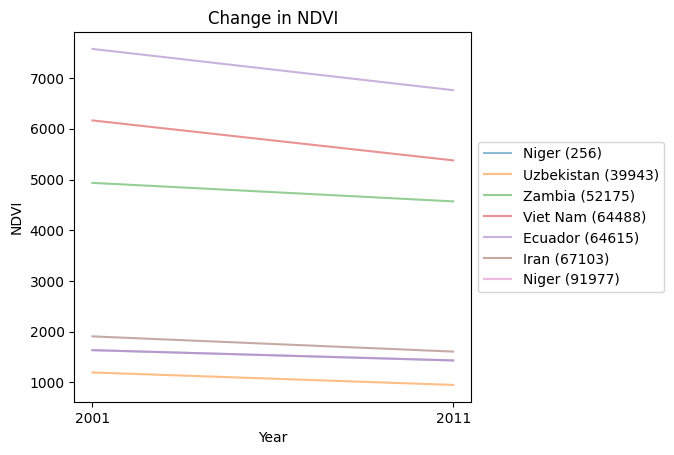
\includegraphics[width=0.7\linewidth]{report/ndvi.png}
    \caption{
        \small
        Plot of NDVI at Chinese financed project sites related to mining in 2001 and 2011.
    }
    \label{fig:ndvi}
\end{figure}



\section{Discussion}

The container developed for the presented use case provides a basic demonstration of how modern industry tools can be leveraged to facilitate research dissemination and replication. While containers can be developed and run on common laptops, they can also easily be deployed on computing clusters using related tools such as Kubernetes. Enabling researchers to share their work in a format that can easily be replicated and extended by others has the potential to improve the uptake of new methods and minimize duplication of efforts in leveraging the latest advancements for applications.

The demonstration presented has already served as a prototype being built upon for AidData's GeoQuery tool. GeoQuery is AidData's free spatial data platform, which enables users to find and aggregate geospatial data from dozens of sources into a single, simple-to-use spreadsheet\citep{Goodman2019}. Containers are now being to used to deploy and run numerous geospatial data pipelines\footnote{See \url{https://github.com/aiddata/geo-datasets}} on a Kubernetes cluster hosted at William \& Mary, which provide the data used in GeoQuery. While these data pipelines run at scale on the Kubernetes cluster to reduce processing times, the underlying containers can be created and run by anyone interested in acquiring the datasets for their own work, regardless of their computational resources. After converting nearly all of the data pipelines supporting GeoQuery to use containers, they can now be run more easily and more frequently to enabled more regular data updates being provided for users. To date, GeoQuery has served over 41,000 data requests to over 8,600 researchers, analysts, and others users at thousands of organizations around the world. 

The development of the use case presented in this report has provided the framework to support considerable ongoing advancements not only within GeoQuery, but also broader research efforts within AidData. Additional researchers within AidData have now been able to leverage the computational resources available within the Kubernetes clusters at William \& Mary by simply preparing containers, without advanced Kubernetes knowledge, that other staff familiar with Kubernetes can deploy and run despite not having knowledge of the specific application running within the container.





\paragraph{Acknowledgements} 

We acknowledge the support of William \& Mary in funding this work through a W\&M Faculty Research Grant, and William \& Mary Research Computing for providing computational resources and/or technical support that have contributed to the results reported. 



\bibliographystyle{apalike}
\bibliography{refs.bib}	

\end{document}